\begin{section}{Fisher Information Content}
  \label{sec:fisherinfo}
  Mathamatically, the Fisher information $I$ of the initial scale
  invariant matter power spectrum, $A$, is defined as
  \begin{align}
    I_A \equiv -\left\langle \frac{\partial ^2 \mathrm{ln \Largr}}{\partial  \mathrm{ln} A ^2}\right\rangle,
    \label{eq:fisherdefine}
  \end{align}
  where $\Largr$ is the likelihood \cite{bib:Tegmark1997}.  
  In this paper, the word \enquote{information} and the symbol \enquote{$I$} both implicitly 
  mean cumulative Fisher information 
  of $A$. For Gaussian
  fields, the likelihood depends on parameters only through the
  power spectrum $P(k)$, so $I$ can be written as 
  \begin{align}
    I = - \left\langle \sum_{k,k'} \frac{\partial \mathrm{ln} P(k)}{\partial \mathrm{ln} A} 
    \frac{\partial ^2 \mathrm{ln \Largr}}{\partial \mathrm{ln} P(k) \partial \mathrm{ln} P(k')}
    \frac{\partial \mathrm{ln} P(k')}{\partial \mathrm{ln} A}\right\rangle,
    \label{eq:fisherdef2}
  \end{align}
  where the angle bracket averages over realizations
  \cite{bib:Rimes2006}.
  Eq.~\ref{eq:fisherdef2} can be written in a simpler
  form in two aspects.   
  
  Firstly, we simplify the derivative term
  $\partial \mathrm{ln} P(k)/\partial\mathrm{ln} A$.  For a given density field $\delta_\alpha$, we can
  conveniently decompose it into a correlated, linear component,
  and an uncorrelated, noise component with respect to $\delta_L$, 
  \begin{align}
    \delta_{\alpha}(k) = r'(k) \delta_L (k) + \delta_{n}(k),
    \label{eq:decompose}
  \end{align}
  where $\delta_{n}(k)$ is defined such that the correlation
  $\langle \delta_L^\dagger(k)\delta_{n}(k) \rangle=0$.  To solve $r'$, we correlate
  both sides with $\delta_L$ and the uncorrelated noise term drops out,
  \begin{align}
    \langle \delta_L^\dagger(k)\delta_\alpha(k) \rangle = r'(k) \langle \delta_L^\dagger(k)\delta_L(k) \rangle.
    \label{eq:correlating}
  \end{align} 
  Using the definitions of cross correlation coefficient, $r_{\alpha L}(k)\equiv P_{\alpha L}/\sqrt{P_{\alpha\alpha}P_{LL}}$ 
  and bias, $b^2(k)\equiv P_{\alpha\alpha}/P_{LL}$, we can solve for $r'$ as
  \begin{align}
    r'(k) = \frac{P_{\alpha L}(k)}{P_{LL}(k)}=r_{\alpha L}(k) b(k).
    \label{eq:bofk}                                              
  \end{align}                                                    
  To find the nonlinear term, we square both sides of Eq.~\ref{eq:decompose}
  and the cross term of the right hand side vanishes,             
  \begin{align}                                                  
    \langle \delta_\alpha^\dagger(k) \delta_\alpha(k) \rangle =  
    r_{\alpha L}^2(k)b^2(k) \langle \delta_L^\dagger(k) \delta_L(k) \rangle + 
    \langle \delta_{n}^\dagger(k)\delta_{n}(k) \rangle,          
  \end{align}                                                    
  and find                                                       
  \begin{align}                                                  
    P_{\alpha\alpha}(k) = r_{\alpha L}^2(k)b^2(k)P_{LL}(k) + P_{nn}(k).
    \label{eq:powerdecompose}                                    
  \end{align}                                                    
  With the help of Eq.~\ref{eq:bofk} and Eq.~\ref{eq:powerdecompose},
  we get                                                         
  \begin{align}                                                  
    \frac{\partial \mathrm{ln} P(k) }{ \partial \mathrm{ln} A}=
    r^2_{\alpha L}(k)b^2(k)\frac{P_{LL}(k)}{P_{\alpha\alpha}(k)}=r^2_{\alpha L}(k).
  \end{align}

  Secondly, we simplify
  $\partial ^2 \mathrm{ln \Largr}/\partial \mathrm{ln} P(k) \partial
  \mathrm{ln} P(k')$
  by using the fact that its expectation value is the Fisher
  matrix.  For Gaussian fields, this is equal to the inverse of the
  covariance matrix which is diagonal with elements given by the
  number of modes in each bin (when considering $\bs{k}$ and $-\bs{k}$ as the same mode).  
  We can extend this definition to
  non-Gaussian fields, by taking into account that the covariance
  matrix is no longer diagonal \cite{bib:Rimes2006}.  Thus, we
  write the Fisher information in terms of matrix multiplication:
  \begin{align}
    I \left( < k_n\right) = r^2(k)^{\mathrm{T}} \left[ \mathrm{C^{-1}_{norm}} 
    ( k,k' )\right]_{<k_n} r^2(k') ,
    \label{eq:fisherformulaused}
  \end{align}
  where
  \begin{align}
    \mathrm{C_{norm}} \left( k,k' \right)=\frac{\mathrm{Cov}(k,k')}
    {\langle P(k)\rangle\langle P(k')\rangle}
  \end{align}
  is the normalized covariance matrix, and
  $r$ is the mean cross correlation of a given density field with
  $\delta_L$ and the subscript $<k_n$ indicates the matrix elements are set to
  zero for modes $k,k'>k_n$.  The covariance matrix is defined as
  \begin{align}
    \mathrm{Cov}\left(k,k'\right)\equiv \frac{\sum_{i,j=1}^{N}\left[ P_i \left( k \right) - 
    \langle P \left( k \right) \rangle \right]\left[ P_j \left( k' \right) - 
    \langle P \left( k' \right)\rangle \right]}{N-1},
  \end{align}
  where $N$ is the total number of simulations and angle bracket average these simulations.  

  The cross-correlation coefficient matrix, or for short the correlation matrix, 
  is defined as 
  \begin{align}
    \mathrm{Corr}\left(k,k'\right)=\frac{\mathrm{Cov}\left(k,k'\right)}
    {\sqrt{\mathrm{Cov}\left(k,k\right)\mathrm{Cov}\left(k',k'\right)}},
  \end{align}
  representing the correlation between different $k$ modes.  The
  correlation matrices for nonlinear and reconstructed power spectra
  are shown in the upper-left and lower-right sections of Fig.~\ref{fig:corrall}.
  By definition, the correlation matrix is symmetric with unit
  diagonal allowing us to overlay the two matrices.  For the
  nonlinear case, it is almost diagonal in the linear
  regime, $k \lesssim 0.07$ $h$/Mpc.  The off-diagonal
  elements are produced by strong mode coupling on nonlinear scales
  and the super-survey tidal effect which is small on linear scales
  but dominates in the weakly nonlinear regime
  \cite{bib:Kazuyuki2016}.  The correlation matrix for the nonlinear
  power spectra has a small amount of negative elements
  ($\mathrm{Corr} \gtrsim -0.18$), which should vanish with more
  simulations \cite{bib:Takahashi2009}.  For the reconstructed
  correlation matrix, the linear regime extends up to $k \simeq 0.3$
  $h$/Mpc.  However, the number and magnitude of negative off-diagonal elements
  also increases ($\mathrm{Corr} \gtrsim -0.49$).

  \begin{figure}
    \centering
    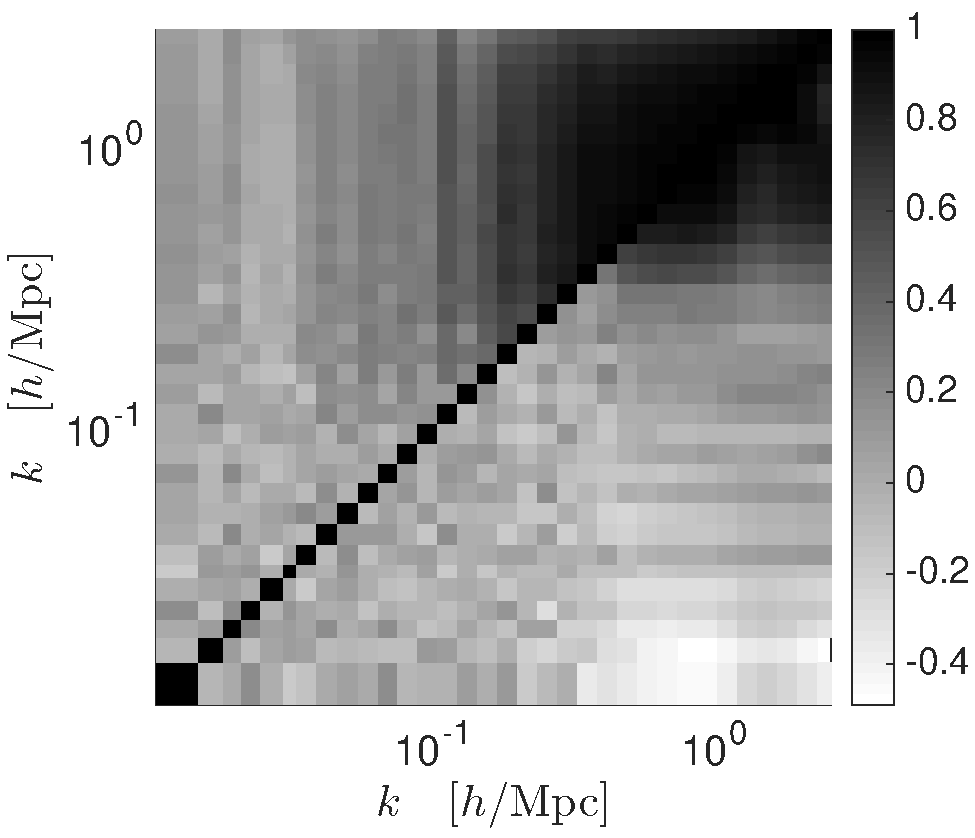
\includegraphics[width=0.48\textwidth]{fig3.pdf}
    \caption{The correlation matrix from 130 nonlinear power
      spectra (the upper triangular elements) and reconstructed power
      spectra (the lower triangular elements).}
    \label{fig:corrall}
  \end{figure}

  The Fisher information is proportional to the volume. 
  We plot the Fisher information per unit volume of the power spectra of
  $\delta_N$, $\delta_L$ and $\delta_R$ in the left panel of 
  Fig.~\ref{fig:fisherinfo}. The Fisher information of the linear 
  power spectra is equal to the cumulative number of $k$-modes, $N_k$. As expected, Fisher information of
  $\delta_N$ decreases from that of $\delta_L$ on scale
  $k \simeq 0.05$ $h$/Mpc, and has a flat plateau on small scales, 
  with a saturated value of
  $I \simeq 2.5 \times 10^{-5}/({\rm Mpc}/h)^3$, indicating
  the absence of independent information in the nonlinear
  regime.  In comparison, the information curve of the $\delta_R$ power
  spectra keeps increasing roughly the same as the linear information
  until $k\simeq 0.3$ $h$/Mpc, and reaches a value of 
  $I \simeq 1.3 \times 10^{-3}/({\rm Mpc}/h)^3$ at $k \simeq 2.7$ $h$/Mpc,
  a factor of 50 times greater than $I_{\delta_N}$.
  As an example to illustrate its strength, we compare the Fisher information given by the MM reconstruction method
  with the logarithmic density mapping method \cite{bib:Mark2009}. We find that MM
  reconstruction gives over 10 times more information.  It also appears to perform 
  significantly better than the standard BAO reconstruction using the Zel'dovich 
  approximation \cite{bib:Ngan2012}, although a direct comparison is left for future work.
  
  To test the upper limit of information that the MM reconstruction can recover, 
  we also checked the Fisher information given by $\delta_E$ \cite{bib:Yu2016} as a reference, 
  which indicates the maximum possible information available via reconstruction procedures.
  We find that $I_{\delta_E}$ is 3 times higher ($150 I_{\delta_N}$) than MM reconstruction.
  This gives motivation to continue to develop and optimize our 
  reconstruction algorithms to achieve this theoretical target.
  
  In some previous works, the cross correlation $r^2$ terms have been set
  to unity in Eq.~\ref{eq:fisherformulaused}, which artificially
  increases the information. To demonstrate this, we plot this case in the right panel of 
  Fig.~\ref{fig:fisherinfo}.  We see that neglecting $r^2$ causes there to be an artificial 
  increase in information on small scales ($k\gtrsim 1h/\mathrm{Mpc}$).  We also see that 
  the information of the logarithmic density
  mapping is much higher than it is in the left panel.  Including the correlation coefficient 
  ensures that the information we compute is that present in the initial conditions and not 
  spuriously induced by the transformation procedure.  This therefore resolves the problems 
  discussed in \cites{bib:HarnoisD2013} \cite{bib:HarnoisD2013} section ``Information about what?''
  We conclude that, in the context of BAO analysis and extracting other primordial cosmological
  parameters, we should take into account the correlation term $r^2$ and
  use Eq.~\ref{eq:fisherformulaused} to compute the Fisher information.
  
  Another way to quantify the nonlinear scale of $\delta_\alpha$
  is via the information plateau's linear equivalent scale, $k_p$, satisfying
  \begin{equation}
      I_{\delta_L}(k_p)=I_{\delta_{\alpha}}(k\rightarrow\infty).
  \end{equation}
  In the left panel of Fig. \ref{fig:fisherinfo}, we can see that 
  $k_p$ is just the scale on which 
  the horizontal dotted line crosses $I_{\delta_{L}}$ curve.
  Practically, we use $I_{\delta_{\alpha}}$ ($k=2.7$ $h$/Mpc)
  as a proxy of $I_{\delta_{\alpha}}(k\rightarrow\infty)$,
  where $k$ is large enough such that $r\rightarrow 0$, ensuring
  the convergence, or saturation of $I_{\delta_{\alpha}}$.
  We find that
  for $\delta_N$, $k_p\simeq 0.15$ $h$/Mpc.
  The MM reconstruction increases $k_p$ to $0.4$ $h$/Mpc,
  whereas the logarithmic density mapping method only increases it to $0.19$ $h$/Mpc.

  \begin{figure*}
    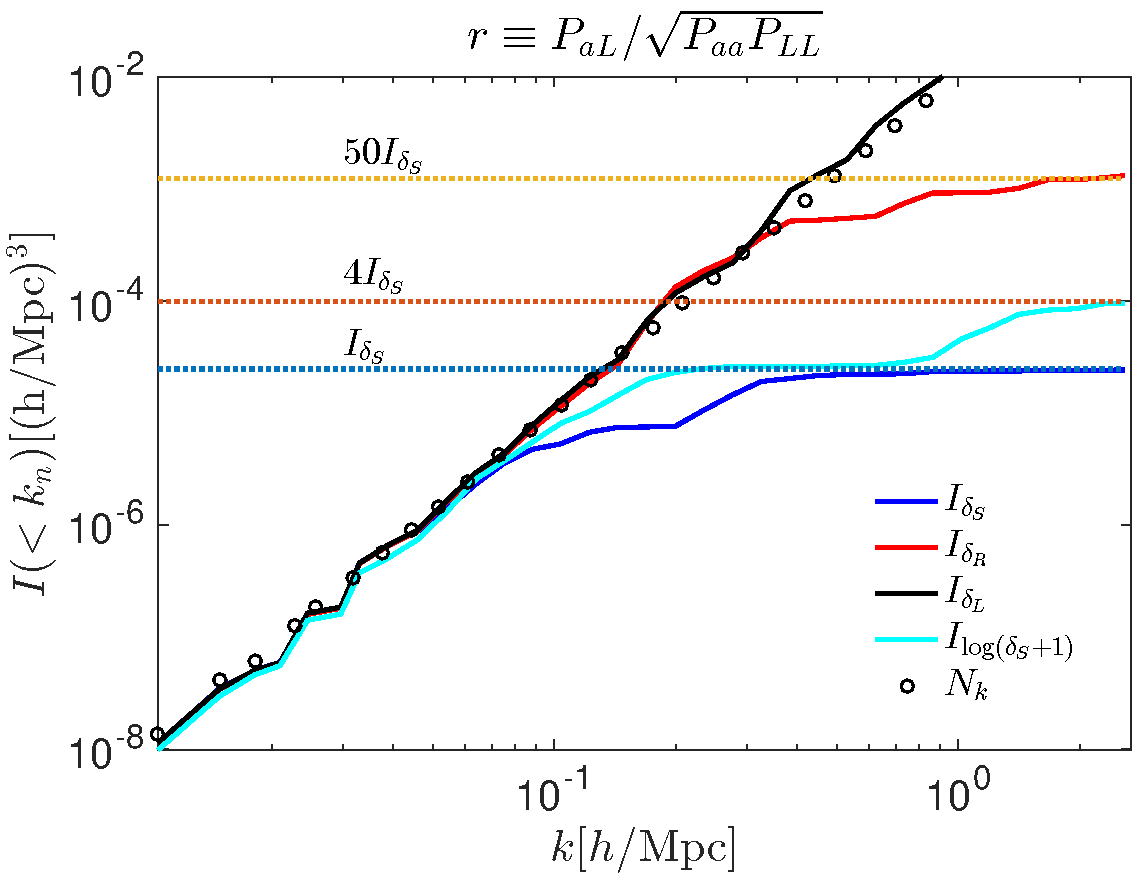
\includegraphics[width=0.48\textwidth]{fig4a.pdf}
    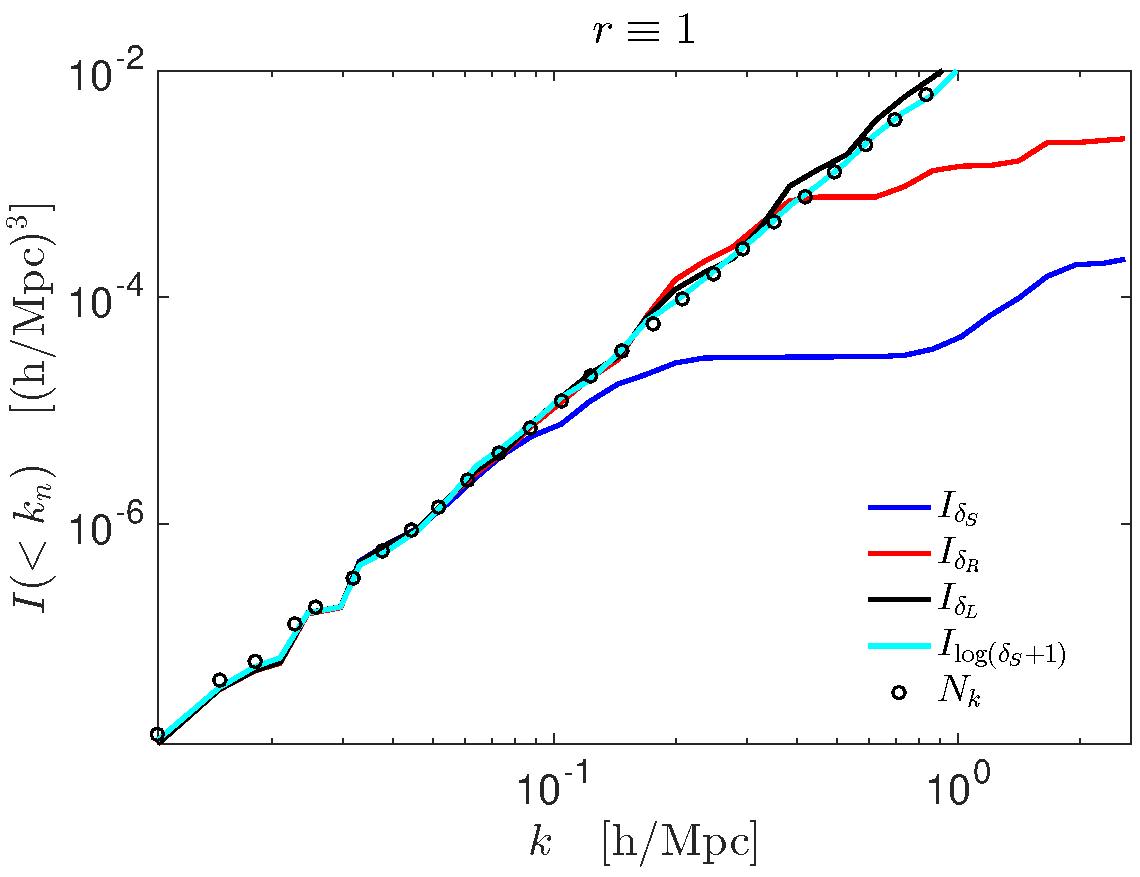
\includegraphics[width=0.48\textwidth]{fig4b.pdf}
    \centering
    \caption{{\it Left.} The Fisher information (solid lines) per unit volume as
      a function of wave number.  The blue, red, and black curves correspond to the power spectra
      of $\delta_N$, $\delta_R$ and $\delta_L$ respectively,
      and the cyan curve
      corresponds to the logarithmic density mapping. The circles
      are the cumulative number of $k$ modes.  Dotted horizontal lines indicate the value of the 
      Fisher information at $k \simeq 2.7$ $h$/Mpc.  {\it Right.} Same
      as the left panel except setting $r\equiv 1$ in Eq.~\ref{eq:fisherformulaused}. The
      black, blue, and cyan lines match the results in \cite{bib:Rimes2006,bib:Mark2009}. 
This naive estimate does not account for the lack of correlation
of the final density field with the initial conditions, and represents
an overestimate of the {\it linear} information.}
  \label{fig:fisherinfo}
\end{figure*}
\end{section}
